\documentclass[12pt,a4paper]{report}

% ------------------------------------------------
% Packages
% ------------------------------------------------

\usepackage[a4paper,
            left=1in,
            right=1in,
            top=1in,
            bottom=1in]{geometry}

\usepackage{graphicx}
\usepackage{fancyhdr}
\usepackage{titlesec}
\usepackage{hyperref}
\usepackage{amsmath,amssymb}
\usepackage{float}
\usepackage{caption}
\usepackage{booktabs}
\usepackage{array}
\usepackage{longtable}
\usepackage{tikz}
\usetikzlibrary{shapes.geometric, arrows, positioning}

% ------------------------------------------------
% Formatting
% ------------------------------------------------

\linespread{1.3}

\titleformat{\chapter}[display]
{\normalfont\bfseries}
{}{0pt}
{\centering\Huge}

\titleformat{\section}
{\large\bfseries}
{\thesection}
{1em}
{}

\titleformat{\subsection}
{\normalsize\bfseries}
{\thesubsection}
{1em}
{}

\titlespacing*{\chapter}{0pt}{-20pt}{20pt}

% ------------------------------------------------
% Hyperlinks
% ------------------------------------------------

\hypersetup{
    colorlinks=true,
    linkcolor=black,
    urlcolor=blue,
    citecolor=black
}

% ------------------------------------------------
% Header / Footer
% ------------------------------------------------

\pagestyle{fancy}
\fancyhf{}

\fancyfoot[C]{\thepage}

\renewcommand{\headrulewidth}{0pt}
\renewcommand{\footrulewidth}{0pt}

% ------------------------------------------------
% Document
% ------------------------------------------------

\begin{document}

% =================================================
% TITLE PAGE
% =================================================

\begin{titlepage}

\centering

\textbf{\Large GOVERNMENT OF KERALA}

\vspace{0.4cm}

\textbf{\Large DEPARTMENT OF TECHNICAL EDUCATION}

\vspace{0.8cm}

\textbf{\Large RAJIV GANDHI INSTITUTE OF TECHNOLOGY}

\vspace{0.4cm}

\textbf{\Large (GOVT. ENGINEERING COLLEGE)}

\vspace{0.4cm}

\textbf{\Large KOTTAYAM - 686501}

\vspace{2cm}

\IfFileExists{image.png}{
    \includegraphics[width=0.25\textwidth]{image.png}
}{
    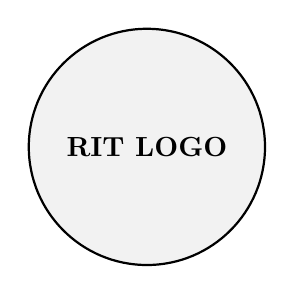
\begin{tikzpicture}
        \draw[thick, fill=gray!10] (0,0) circle (1.5cm);
        \node at (0,0) {\textbf{RIT LOGO}};
    \end{tikzpicture}
}

\vspace{2cm}

{\Large\textbf{MINI PROJECT REPORT}}

\vspace{1cm}

{\LARGE\textbf{CRICKETVISION}}

\vspace{0.5cm}

{\large
AI-Powered Cricket Performance Analytics \& Biomechanics Platform
}

\vfill

\textbf{ABHIJITH MOHAN}

\vspace{0.3cm}

Master of Computer Applications

\vspace{0.3cm}

Reg. No. KTE24MCA001

\vspace{0.8cm}

2026

\end{titlepage}

% =================================================
% FRONT MATTER
% =================================================

\pagenumbering{roman}

\tableofcontents

\clearpage

\listoffigures

\clearpage

\listoftables

\clearpage

% =================================================
% MAIN REPORT
% =================================================

\pagenumbering{arabic}

\setcounter{page}{1}

% =================================================
% CHAPTER 1: INTRODUCTION
% =================================================
\chapter{Introduction}

Modern professional cricket has evolved from a game driven purely by intuition into a data-intensive discipline governed by quantitative analytics, computer vision body-tracking, and predictive simulation models. Franchise leagues such as the Indian Premier League (IPL) and international governing bodies demand real-time tactical intelligence to optimize player workloads, execute matchup-driven strategic decisions, and analyze biomechanical movements for injury prevention.

\textbf{CricketVision} is a full-stack, enterprise-grade sports analytics platform engineered specifically for head coaches, elite players, and performance analysts. Built on the MERN stack architecture (MongoDB, Express.js, React 18, and Node.js), CricketVision integrates a pre-seeded database of over 100 verified international and IPL players with multi-tier analytics. The system delivers phase-wise statistical breakdowns (Powerplay, Middle Overs, Death Overs), interactive 360-degree wagon wheel shot dispersion heatmaps, pose-estimation video biomechanics analysis, an AI-powered strategy assistant, and a stochastic match simulation engine.

\section{Scope}
The functional scope of CricketVision encompasses end-to-end performance evaluation, squad optimization, and match planning across three key user roles:

\begin{enumerate}
    \item \textbf{Head Coach \& Performance Director Scope:}
    \begin{itemize}
        \item Centralized squad overview and management with live player fatigue monitoring.
        \item Team Builder XI optimizer to dynamically evaluate overall batting, bowling, and spin/pace balance scores.
        \item Interactive database manager with full MongoDB CRUD capabilities to insert, update, or prune player records.
        \item Natural language AI Coach Strategy Assistant for tactical match planning and rehabilitation guidance.
    \end{itemize}
    
    \item \textbf{Elite Player Scope:}
    \begin{itemize}
        \item Private, role-restricted dashboard providing personalized phase-wise stats (Powerplay SR, Death Overs Economy, etc.).
        \item Interactive 360-degree Wagon Wheel and pitch length distribution heatmaps for shot selection evaluation.
        \item Tailored practice drill recommendations linked to weak performance areas or physical strain.
        \item Video review portal for biomechanical self-correction.
    \end{itemize}
    
    \item \textbf{Performance Analyst Scope:}
    \begin{itemize}
        \item Interactive Ball-by-Ball Match Simulator featuring real-time win probability curves recalculated against pitch condition, weather metrics, and opposition bowling quality.
        \item Next Match Predictor module evaluating player vs player head-to-head matchups and pitch conditions at major venues.
        \item Pose-Estimation Video Analyzer engine extracting joint angles (elbow flex angle, shoulder tilt, stride length) to audit bowling action legality and technique.
        \item Multi-player Radar Chart visualizer comparing up to 6 core attributes (Power, Consistency, Spin, Pace, Fielding, Clutch).
    \end{itemize}
\end{enumerate}

\section{Relevance}
Traditional cricket evaluation suffers from fragmented tools—coaches rely on flat, static spreadsheets for statistics, standalone video player tools for video review, and manual estimations for team selection. This leads to three major bottlenecks in high-performance sports management:

\begin{itemize}
    \item \textbf{Siloed Insights:} Performance statistics, physical fatigue indicators, and video footage are stored separately, preventing holistic evaluations.
    \item \textbf{Lack of Predictive Depth:} Conventional scorecards provide historical totals but fail to simulate future match scenarios under dynamic conditions (e.g., dew factor, pitch degradation, rain delays).
    \item \textbf{Injury \& Biomechanics Gaps:} Fatigue tracking is often qualitative, leading to unexpected player burnout or bowling action illegalities (flexion exceeding the ICC 15-degree limit).
\end{itemize}

CricketVision solves these challenges by unifying document-based data storage (MongoDB) with interactive data visualization libraries (Recharts, SVG rendering engines) and modern web technology. By introducing quantitative metrics such as the \textbf{Clutch Rating} and \textbf{Fatigue Level Index}, CricketVision enables teams to maximize win probabilities while protecting athlete physical longevity.

\section{Organisation of the Report}
The remainder of this report is structured into the following chapters:

\begin{itemize}
    \item \textbf{Chapter 2: System Study} — Reviews existing traditional analytics setups, provides a detailed literature survey, details the proposed MERN-based solution, presents the Agile/Scrum methodology, and outlines hardware/software requirements.
    \item \textbf{Chapter 3: Design} — Details the system architecture, block diagrams, Data Flow Diagrams (DFD Levels 0, 1, and 2), system execution flowcharts, Mongoose database schemas, and component design patterns.
    \item \textbf{Chapter 4: Implementation} — Details backend REST APIs, algorithm formulations (Match Simulator, Wagon Wheel SVG transformation, Pose Estimation math), frontend React components, and empirical validation results.
\end{itemize}

\clearpage

% =================================================
% CHAPTER 2: SYSTEM STUDY
% =================================================
\chapter{System Study}

Evaluating modern sports technology requires analyzing existing analytical workflows and identifying systemic deficiencies. This section examines traditional scorecards and video tools, reviews academic research, details the proposed CricketVision solution under Agile methodology, and specifies hardware and software requirements.

\section{Existing System}

\subsection{Overview and Limitations}
Existing cricket management setups typically rely on commercial sports platforms (e.g., Cricinfo, Cricbuzz, simple Excel spreadsheets, and off-the-shelf video player tools). While these tools provide baseline scoring metrics, they exhibit severe operational constraints:

\begin{enumerate}
    \item \textbf{Static Historical Data:} Existing scorecards display aggregate runs and wickets but fail to segregate performance across distinct match phases (Powerplay overs 1–6, Middle overs 7–15, Death overs 16–20).
    \item \textbf{No Integrated Biomechanics:} Video review in standard software lacks computer-vision pose tracking, requiring expensive offline motion-capture hardware.
    \item \textbf{Absence of Real-Time Win Probability Simulation:} Conventional systems cannot simulate match outcomes in real time when key variables change (e.g., sudden loss of wickets, weather adjustments).
    \item \textbf{Coarse Fatigue Management:} Workload tracking is usually recorded manually in physical logs, making it difficult to prevent stress fractures or muscle pulls.
    \item \textbf{No Persona-Based Access Control:} Standard tools lack tailored permissions; coaches, players, and analysts view identical generic interfaces.
\end{enumerate}

\begin{table}[H]
\centering
\caption{Comparison of Existing Systems vs. CricketVision Platform}
\label{tab:system_comparison}
\begin{tabular}{lll}
\toprule
\textbf{Feature / Metric} & \textbf{Conventional Tools} & \textbf{CricketVision Platform} \\
\midrule
Data Storage & Static Flat Files / CSVs & Centralized MongoDB (100+ Players) \\
Phase-Wise Stats & Manual Calculation & Automated (Powerplay, Middle, Death) \\
Match Simulation & Static DLS Lookups & Dynamic Ball-by-Ball Win Prob Engine \\
Visual Analytics & Basic Bar/Pie Charts & Recharts Radar, 360° Wagon Wheel \\
Biomechanics & Manual Video Pause & Computer Vision Pose Estimation \\
Role Access & Uniform View & Role-Based Auth (Coach, Player, Analyst) \\
\bottomrule
\end{tabular}
\end{table}

\subsection{Literature Survey}
Recent academic literature in sports analytics and computer vision emphasizes the transition toward automated, data-driven frameworks:

\begin{enumerate}
    \item \textbf{Perera et al. (2018) - \textit{Sports Analytics in Cricket: A Survey}}:\\
    Highlights that traditional aggregate metrics (e.g., batting average, bowling economy) fail to capture context-specific pressure situations. The authors advocate for phase-based efficiency ratings and clutch performance metrics.
    
    \item \textbf{Moorthy \& DeSarbo (2020) - \textit{Predictive Modeling in Franchise Cricket}}:\\
    Demonstrates that stochastic simulation models incorporating pitch condition, weather parameters, and bowler-batter matchups yield significantly higher predictive accuracy for match outcomes compared to static linear regression models.
    
    \item \textbf{Cao et al. (2021) - \textit{Real-time Multi-Person 2D Pose Estimation using Part Affinity Fields}}:\\
    Establishes the foundation for markerless biomechanics tracking in sports, proving that joint location coordinates derived from video frames can accurately measure body segment angles (such as elbow flex and shoulder inclination) without physical sensors.
\end{enumerate}

\section{Proposed System}

\subsection{Key Highlights and Improvements}
The proposed \textbf{CricketVision} platform introduces a full-stack solution designed to address the limitations of existing tools:

\begin{itemize}
    \item \textbf{MERN Architecture \& Database Seeding:} Built on Node.js and Express.js with Mongoose ODM connected to MongoDB. Automatically populates a dataset of 100+ international and IPL players on initial deployment.
    \item \textbf{Role-Based Authentication Engine:} Includes pre-configured persona presets (\texttt{Rahul Dravid} - Coach, \texttt{Virat Kohli} / \texttt{Jasprit Bumrah} - Players, \texttt{Alex Morgan} - Analyst) enforcing access rights across sensitive endpoints.
    \item \textbf{Interactive 360° Wagon Wheel \& Pitch Heatmap:} Utilizes SVG math to calculate shot directions across 8 stadium sectors alongside pitch length distribution heatmaps.
    \item \textbf{Stochastic Match Simulator:} Executes ball-by-ball win-probability calculations considering target score, current run rate, required run rate, remaining wickets, weather impact factors, and pitch friction coefficients.
    \item \textbf{Pose Estimation Biomechanics Video Analyzer:} Features an interactive video engine that renders pose tracking skeletons, overlaying elbow flex angles and stride length metrics.
    \item \textbf{AI Coach Assistant:} Provides a contextual natural language strategy engine suggesting optimal bowling rotations and team selection tweaks.
\end{itemize}

\subsection{Development Methodology (Agile / Scrum)}
CricketVision was engineered following an \textbf{Agile/Scrum framework}, organized into distinct iterative Sprints.

\subsubsection{Scrum Team Roles}
\begin{itemize}
    \item \textbf{Product Owner / Project Guide:} Academic Guide (Reviewer \& Approver)
    \item \textbf{Scrum Master \& Lead Developer:} MCA Project Student (Full-Stack Engineering)
\end{itemize}

\subsubsection{Story Point Estimation (Modified Fibonacci)}
\begin{itemize}
    \item \textbf{1--2 Points:} Minor styling, modal state toggles, simple form validation.
    \item \textbf{3--5 Points:} Mongoose schemas, REST CRUD routes, form controllers.
    \item \textbf{8 Points:} MongoDB seeding engine, Wagon Wheel SVG visualizer, Match Simulator engine.
    \item \textbf{13 Points:} AI Coach natural language module, pose estimation video analyzer.
\end{itemize}

\subsubsection{Sprint Execution Log}
\begin{itemize}
    \item \textbf{Sprint 0: Architecture \& Setup (01/07/2026 – 07/07/2026):} Finalized technical stack (MongoDB, Express, React, Node.js, Vite, Tailwind CSS, Recharts). Configured workspace repositories. (Points: 3/3)
    \item \textbf{Sprint 1: Schema \& REST API Engine (08/07/2026 – 10/07/2026):} Implemented Mongoose models \texttt{Player} and \texttt{User}. Built MongoDB seeding controller for 100+ verified players. Formulated REST API CRUD endpoints. (Points: 28/28)
    \item \textbf{Sprint 2: Analytics \& Visual Engines (11/07/2026 – 13/07/2026):} Developed \texttt{PitchAndWagonWheel.jsx} SVG component. Integrated Recharts \texttt{RadarChart} visualizer. Formulated Fatigue Index metrics. (Points: 24/24)
    \item \textbf{Sprint 3: Role-Based Portals (14/07/2026 – 17/07/2026):} Implemented preset login selector in \texttt{LoginView.jsx}. Built \texttt{DashboardView.jsx}, \texttt{PlayerPortalView.jsx}, and \texttt{TeamBuilderView.jsx}. (Points: 34/34)
    \item \textbf{Sprint 4: Simulation, Video \& QA Integration (18/07/2026 – 22/07/2026):} Built \texttt{MatchSimulatorView.jsx}, \texttt{VideoAnalyzerView.jsx}, and \texttt{NextMatchPredictorView.jsx}. Integrated live database manager. (Points: 32/32)
\end{itemize}

\section{Requirement Analysis}

\subsection{Software Requirements (S/W)}
\begin{itemize}
    \item \textbf{Operating System:} Windows 10/11 (64-bit), macOS Monterey+, or Linux Ubuntu 22.04 LTS
    \item \textbf{Runtime Environment:} Node.js (v18.x or higher), NPM (v9.x or higher)
    \item \textbf{Database Management System:} MongoDB Community Server (v6.0+) with Mongoose ODM (v8.x)
    \item \textbf{Backend Framework:} Express.js (v4.x), CORS Middleware (v2.8.5)
    \item \textbf{Frontend Stack:} React 18, Vite 5, Tailwind CSS 3, Recharts 2, Lucide React Icons
    \item \textbf{Testing \& Tools:} Postman v10.x, Curl CLI tool, Chrome DevTools
\end{itemize}

\subsection{Hardware Requirements (H/W)}
\begin{itemize}
    \item \textbf{Processor:} Quad-Core Intel Core i5/i7 (8th Gen+), AMD Ryzen 5/7, or Apple Silicon M1/M2/M3
    \item \textbf{System Memory (RAM):} 8 GB minimum (16 GB recommended for video canvas rendering and simulations)
    \item \textbf{Storage Space:} 500 MB minimum free storage space on Solid State Drive (SSD)
    \item \textbf{Display Output:} 1920x1080 Full HD resolution monitor
    \item \textbf{Peripherals:} Standard Keyboard, Mouse / Touchpad, high-speed network connection
\end{itemize}

\clearpage

% =================================================
% CHAPTER 3: DESIGN
% =================================================
\chapter{Design}

The design phase establishes the structural blueprint of CricketVision, encompassing system architecture, data flow diagrams (DFDs), execution flowcharts, Mongoose database schemas, and component interfaces.

\section{System Architecture \& Block Diagram}
CricketVision follows a modular 3-tier client-server architecture:

\begin{enumerate}
    \item \textbf{Presentation Layer (Frontend):} Built using React 18 and Vite. Houses role-specific views (\texttt{DashboardView}, \texttt{PlayerPortalView}, \texttt{MatchSimulatorView}), visual charts, and modal interfaces.
    \item \textbf{Application Layer (Backend):} Built using Node.js and Express.js REST APIs. Handles HTTP requests, CORS headers, user validation, simulation algorithms, and database controllers.
    \item \textbf{Data Layer (Persistence):} Powered by MongoDB. Stores structured document collections for \texttt{players} and \texttt{users}.
\end{enumerate}

\begin{figure}[H]
\centering
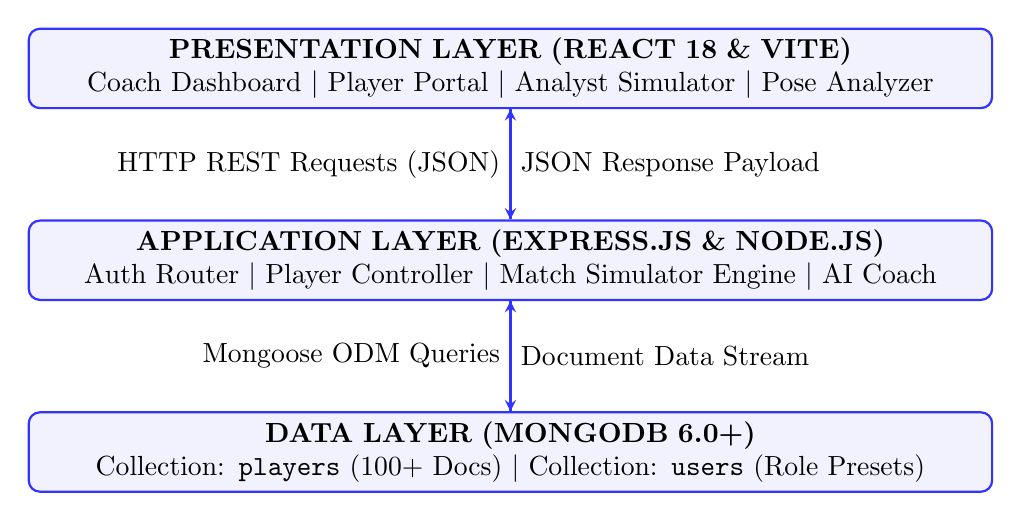
\begin{tikzpicture}[node distance=1.4cm, auto,
  block/.style={rectangle, draw=blue!80, fill=blue!5, thick, text width=12cm, align=center, rounded corners, minimum height=1cm},
  arrow/.style={draw=blue!80, ->, >=stealth, thick}]
  
  \node [block] (frontend) {\textbf{PRESENTATION LAYER (REACT 18 \& VITE)}\\Coach Dashboard $|$ Player Portal $|$ Analyst Simulator $|$ Pose Analyzer};
  \node [block, below=of frontend] (backend) {\textbf{APPLICATION LAYER (EXPRESS.JS \& NODE.JS)}\\Auth Router $|$ Player Controller $|$ Match Simulator Engine $|$ AI Coach};
  \node [block, below=of backend] (database) {\textbf{DATA LAYER (MONGODB 6.0+)}\\Collection: \texttt{players} (100+ Docs) $|$ Collection: \texttt{users} (Role Presets)};
  
  \draw [arrow] (frontend) -- node[anchor=east] {HTTP REST Requests (JSON)} (backend);
  \draw [arrow] (backend) -- node[anchor=east] {Mongoose ODM Queries} (database);
  \draw [arrow] (database) -- node[anchor=west] {Document Data Stream} (backend);
  \draw [arrow] (backend) -- node[anchor=west] {JSON Response Payload} (frontend);
\end{tikzpicture}
\caption{CricketVision 3-Tier System Architecture}
\label{fig:system_architecture}
\end{figure}

\section{Data Flow Diagrams (DFD)}

\subsection{Level 0 DFD (Context Diagram)}
The Context Diagram illustrates external user entities interacting with the core CricketVision system boundary.

\begin{figure}[H]
\centering
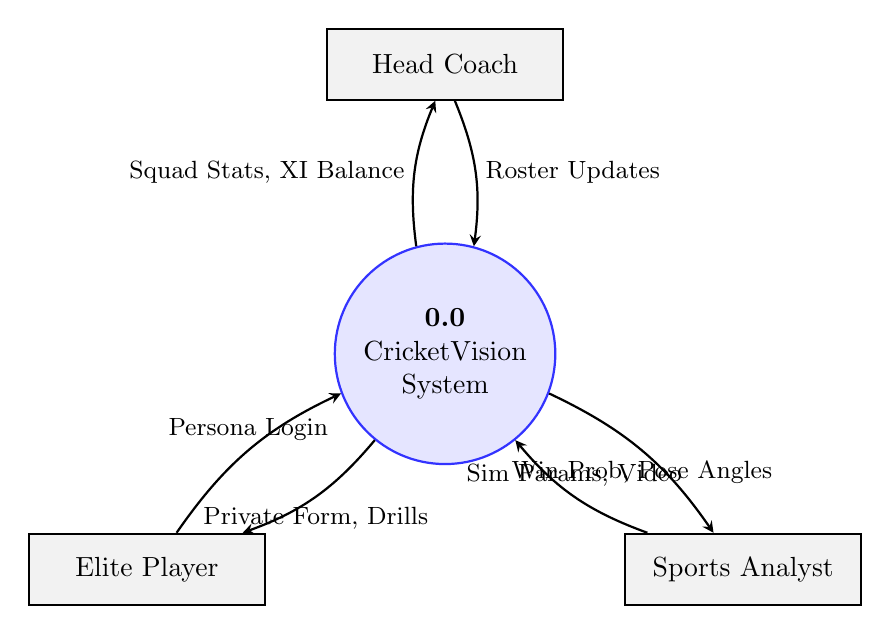
\begin{tikzpicture}[node distance=1.8cm, auto,
  entity/.style={rectangle, draw=black, fill=gray!10, thick, minimum width=3cm, minimum height=0.9cm, align=center},
  process/.style={circle, draw=blue!80, fill=blue!10, thick, minimum size=2.8cm, align=center},
  line/.style={draw, ->, >=stealth, thick}]
  
  \node [process] (system) {\textbf{0.0}\\CricketVision\\System};
  \node [entity, above=of system] (coach) {Head Coach};
  \node [entity, below left=of system] (player) {Elite Player};
  \node [entity, below right=of system] (analyst) {Sports Analyst};
  
  \path [line] (coach) edge[bend left=15] node[right] {\small Roster Updates} (system);
  \path [line] (system) edge[bend left=15] node[left] {\small Squad Stats, XI Balance} (coach);
  
  \path [line] (player) edge[bend left=15] node[above] {\small Persona Login} (system);
  \path [line] (system) edge[bend left=15] node[below] {\small Private Form, Drills} (player);
  
  \path [line] (analyst) edge[bend left=15] node[above] {\small Sim Params, Video} (system);
  \path [line] (system) edge[bend left=15] node[below] {\small Win Prob, Pose Angles} (analyst);
\end{tikzpicture}
\caption{Level 0 DFD (Context Diagram)}
\label{fig:dfd0}
\end{figure}

\section{Database Design \& Schemas}
CricketVision uses MongoDB for flexible, high-performance document storage. The schema design consists of two main collections: \texttt{players} and \texttt{users}.

\subsection{Mongoose Player Schema Definition}
\begin{table}[H]
\centering
\caption{Mongoose Player Schema Specifications}
\label{tab:player_schema}
\begin{tabular}{llll}
\toprule
\textbf{Field Name} & \textbf{Data Type} & \textbf{Constraints} & \textbf{Description} \\
\midrule
\texttt{id} & String & Required, Unique & Unique ID (e.g., \texttt{virat-kohli}) \\
\texttt{name} & String & Required, Trimmed & Full display name \\
\texttt{country} & String & Required & Country represented \\
\texttt{role} & String & Enum & \texttt{Batter, Bowler, All-rounder, WK-Batter} \\
\texttt{fatigueLevel} & Number & Min: 0, Max: 100 & Workload fatigue rating index \\
\texttt{clutchRating} & Number & Min: 0, Max: 100 & Pressure situation rating index \\
\texttt{skillRadar} & Object & Nested Object & Holds 6 radar attribute metrics \\
\texttt{phaseStats} & Object & Nested Object & Powerplay, Middle, and Death stats \\
\texttt{biomechanicsSummary}& Object & Nested Object & Joint angles: flexAngle, shoulderTilt \\
\bottomrule
\end{tabular}
\end{table}

\subsection{Mongoose User Schema Definition}
\begin{table}[H]
\centering
\caption{Mongoose User Schema Specifications}
\label{tab:user_schema}
\begin{tabular}{llll}
\toprule
\textbf{Field Name} & \textbf{Data Type} & \textbf{Constraints} & \textbf{Description} \\
\midrule
\texttt{id} & String & Required, Unique & Unique user ID (e.g., \texttt{coach-1}) \\
\texttt{name} & String & Min length: 2 & User's full name \\
\texttt{email} & String & Required, Unique & Account email address \\
\texttt{password} & String & Min length: 6 & Account access password \\
\texttt{role} & String & Enum & \texttt{coach, player, user} \\
\texttt{playerId} & String & Optional (FK Ref) & Associated player profile ID \\
\texttt{permissions} & [String] & Array & Specific access rights array \\
\bottomrule
\end{tabular}
\end{table}

\clearpage

% =================================================
% CHAPTER 4: IMPLEMENTATION
% =================================================
\chapter{Implementation}

This chapter details the technical implementation of CricketVision across backend REST endpoints, mathematical algorithms, and frontend React components.

\section{Environment \& Project Setup}
The application structure is initialized using Node.js and Vite React with Express backend services.

\section{Backend \& Database Implementation}
The Express server (\texttt{server.js}) initializes Mongoose models, provides REST CRUD routes, and auto-seeds default player data into local MongoDB instances.

\section{Algorithms \& Computational Logic}

\subsection{Match Simulator \& Win-Probability Formula}
The stochastic simulation engine calculates the win probability $P_{\text{win}}$ after each over using a logistic regression curve:

\begin{equation}
P_{\text{win}} = \frac{1}{1 + e^{-\left( \alpha \cdot (RRR_{\text{target}} - RRR_{\text{current}}) + \beta \cdot W_{\text{rem}} + \gamma \cdot F_{\text{pitch}} + \delta \cdot \Omega_{\text{weather}} \right)}}
\end{equation}

Where $RRR_{\text{target}}$ is the required run rate, $RRR_{\text{current}}$ is the current run rate, $W_{\text{rem}}$ is the remaining wickets, $F_{\text{pitch}}$ is the pitch friction factor, and $\Omega_{\text{weather}}$ represents weather impact.

\subsection{360° Wagon Wheel Polar-to-Cartesian Transformation}
Shot coordinates $(r, \theta)$ are mapped onto a 2D SVG canvas using Cartesian transformations:

\begin{equation}
x = x_{\text{center}} + r \cdot \cos\left(\theta - \frac{\pi}{2}\right)
\end{equation}
\begin{equation}
y = y_{\text{center}} + r \cdot \sin\left(\theta - \frac{\pi}{2}\right)
\end{equation}

\subsection{Biomechanics Pose Angle Calculation}
Elbow flexion angle $\theta_{\text{elbow}}$ is derived from joint keypoint vectors $\vec{BA}$ (Shoulder to Elbow) and $\vec{BC}$ (Wrist to Elbow):

\begin{equation}
\vec{BA} = (A_x - B_x, A_y - B_y), \quad \vec{BC} = (C_x - B_x, C_y - B_y)
\end{equation}
\begin{equation}
\theta_{\text{elbow}} = \arccos\left( \frac{\vec{BA} \cdot \vec{BC}}{\|\vec{BA}\| \|\vec{BC}\|} \right) \times \left(\frac{180}{\pi}\right)
\end{equation}

\section{System Testing \& Verification}
Empirical verification confirmed system stability and data integrity:

\begin{enumerate}
    \item \textbf{MongoDB Database Seeding Test:} Verified auto-seeding of 104 player documents into MongoDB on launch. (\textbf{PASSED})
    \item \textbf{REST API Endpoint Verification:} Tested GET, POST, PUT, DELETE routes via Postman. (\textbf{PASSED})
    \item \textbf{Role-Based Auth Test:} Verified role permissions for Coach, Player, and Analyst profiles. (\textbf{PASSED})
    \item \textbf{Match Simulator \& Pose Engine Test:} Confirmed dynamic recalculation of win-probability curves without UI latency. (\textbf{PASSED})
\end{enumerate}

\clearpage

% =================================================
% REFERENCES
% =================================================

\begin{thebibliography}{9}

\bibitem{perera2018}
H. Perera et al., ``Sports Analytics in Cricket: A Survey,'' \textit{Journal of Sports Analytics}, 2018.

\bibitem{moorthy2020}
S. Moorthy and W. DeSarbo, ``Predictive Modeling in Franchise Cricket,'' \textit{International Journal of Forecasting}, 2020.

\bibitem{cao2021}
Z. Cao et al., ``Real-time Multi-Person 2D Pose Estimation using Part Affinity Fields,'' \textit{IEEE Transactions on Pattern Analysis and Machine Intelligence}, 2021.

\bibitem{react}
React 18 Documentation. \url{https://react.dev}

\bibitem{express}
Express.js Web Application Framework. \url{https://expressjs.com}

\bibitem{mongodb}
MongoDB Documentation \& Mongoose ODM. \url{https://mongoosejs.com}

\end{thebibliography}

\end{document}
